\graphicspath{{Others/}}

\section{Déroulement du projet}
\subsection{Organisation théorique du travail}
\subsubsection{Répartition des tâches et prévision de l'emploi du temps}
Le projet fut dès le départ pensé dans le but d'être simple à séparer sous formes de modules, permettant de travailler en parallèle sur plusieurs fonctionnalités.
De plus nous comme nous avions nous même proposé le sujet, il fut assez difficile de prévoir une charge de travail associée à chaque module. Nous avons donc estimé 
de manière très grossière le temps de travail par module. Pour être sûr de pouvoir ajuster le déroulement du projet, nous avons prévus des modules de durées différentes permettant ainsi
de choisir un module en fonction du temps restant, c'est pour cette raison que la durée estimée est supérieure au 60H par personne que nous sommes censés faire.
\par
Nous avions prévu, lors de notre premier rendez-vous avec notre tuteur, de travailler 4H par semaine de cours et de ne pas travailler les semaines de vacances.
Nous avons sommes donc parvenu à finaliser l'emploi du temps suivant, qui n'avait pas pour but d'être suivis à la lettre.
\vfill
\begin{figure}[!h]
    \begin{center}
        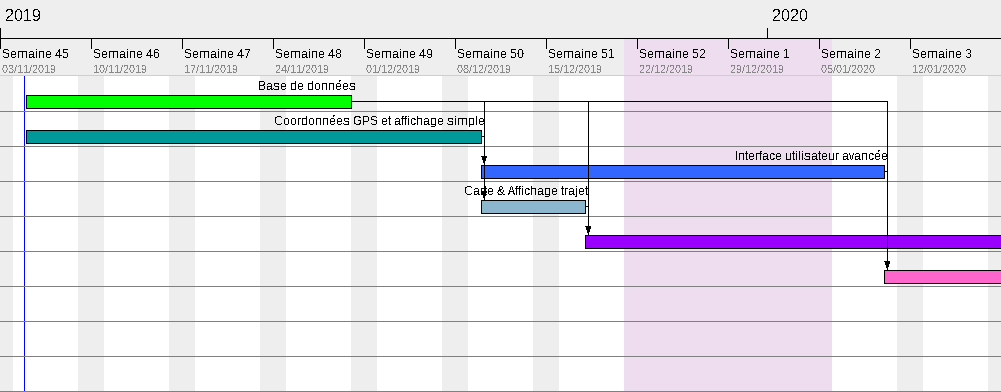
\includegraphics[height=6cm]{test-1.png}
        \caption{Première partie du diagramme de Gantt prévisionnel}
    \end{center}
\end{figure}
\subsubsection{Explications sur les tâches}
Les deux premiers objectifs fixés étaient assez simples, leur but étaient de nous laisser le temps d'être à l'aise avec les technologies choisies.
Nous devions prévoir la base de données, c'est à dire la concevoir et la mettre en place sur la machine virtuelle. En parallèle de celà, nous devions réussir à récupérer les coordonnées GPS du téléphone, et réussir à les afficher.
\par
Les objectifs suivant étaient d'enrichir l'expérience utilisateur en améliorant l'interface. Nous voulions en premier permettre la gestion d'un compte utilisateur depuis l'application, ce qui implique un écran de connexion, un écran de création de compte ainsi qu'un écran de gestion de compte.
Dans un second point (développé en parallèle) nous devions enrichir l'interface fonctionnelle de l'application, c'est à dire insérer une interface contenant une carte sur laquelle notre trajet serait affichable (celà sous entend de stocker les coordonnées aquises).
\par
Nous avions prévus de faire évoluer l'application en rajoutant du contenu. Il aurait fallu ajouter des statistiques plus complètes sur les trajets effectués, comme par exemple$\ :$ le dénivelé, la météo ou bien une estimation des calories dépensées.
Il fallait également introduire une gestion des utilisateurs plus développée, qui permettrait de gérer plus finement les droits d'accès. On aurait ainsi pu dire qu'un autre utilisateur avait participé à un trajet, ou bien qu'il avait le droit d'en modifier le contenu.
De la même manière, on aurait pû créer des groupes d'utilisateurs pour un club par exemple. Dans ces groupes tout le monde aurait accès en lecture uniquement sauf les administrateurs. Ainsi un club sportif aurait pû utiliser l'application pour organiser des séances de randonnées.
\par
Un des derniers points à mettre en place était l'affichage des statistiques précédemments acquises sous la forme de graphique où l'on aurait pu choisir l'échelle, et les trajets qui rentraient en compte.
Le dernier point était radicalement plus difficile à traiter, nous voulions finir le développement de l'application en la faisant se rapprocher d'un réseau social. On aurait alors pu avoir des amis, un fils d'actualité contenant les trajets (publiques) de nos amis. On aurait aussi pu partager
nos trajets via des liens webs, qui auraient été ouvrables uniquement par notre application.
\par
Enfin il y avait la dernière tâche qui semble évidente qui était la rédaction du rapport. Nous avions prévu de prendre des notes au fur et à mesure du développement du projet pour parvenir à rédiger le rapport plus efficacement.
\vfill
\begin{figure}[!h]
    \begin{center}
        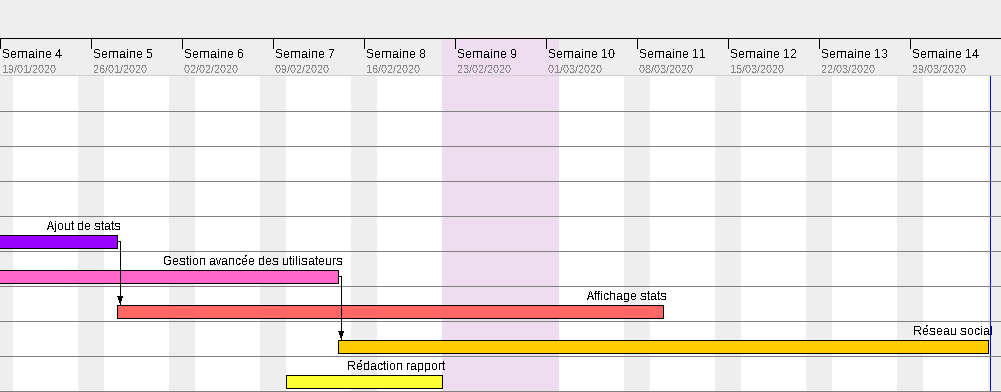
\includegraphics[height=6cm]{test-2.png}
        \caption{Seconde partie du diagramme de Gantt prévisionnel}
    \end{center}
\end{figure}






\subsection{Organisation réelle du travail}
\subsubsection{Répartion des tâches et emploi du temps}
    A la place de débuter le projet comme prévu : chacun sur un module, nous avons préférés faire quelques séances de travail en commun afin de découvrir ensemble l'environnement android, et de nous mettre entièrement d'accord sur ce que nous voulions faire par la suite.
\par
\vfill
\begin{figure}[!h]
    \begin{center}
        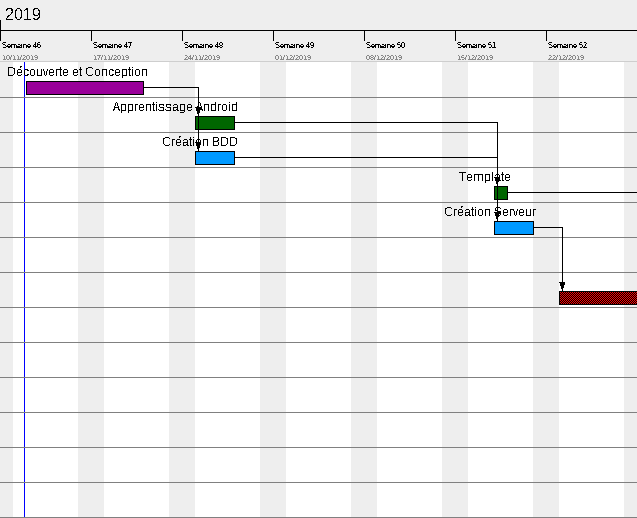
\includegraphics[height=7.5cm]{reel-1.png}
        \caption{Première partie du diagramme de Gantt réel}
    \end{center}
\end{figure}
\newpage
fefe
\vfill
\begin{figure}[!h]
    \begin{center}
        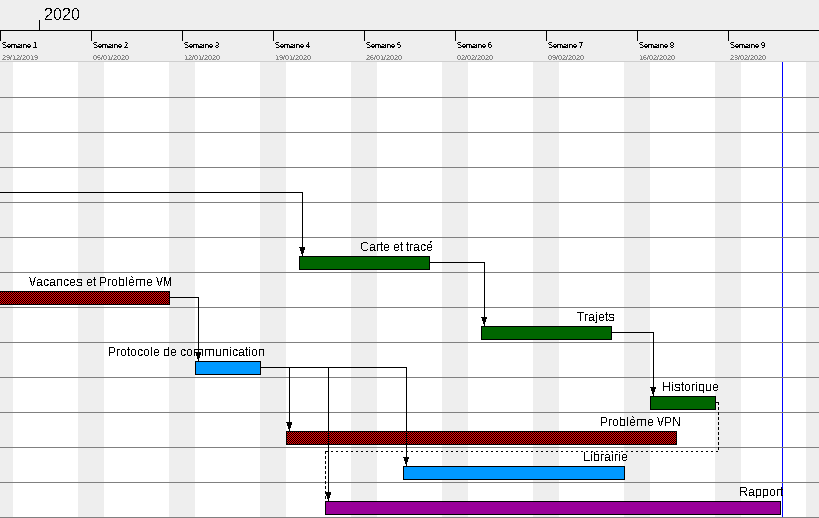
\includegraphics[height=7.5cm]{reel-2.png}
        \caption{Seconde partie du diagramme de Gantt réel}
    \end{center}
\end{figure}
\newpage
\subsubsection{Explications sur les tâches}




\subsection{Problèmes rencontrés}

